\documentclass[fleqn,10pt]{wlscirep}
\usepackage[utf8]{inputenc}
\def\precdot{\mathbin{<\kern-1.5ex\raisebox{0pt}{$\cdot$}}}
\newcommand{\myop}[1]{\ensuremath{\mathop{\mathrm{#1}}\nolimits}}
\newcommand{\est}{\myop{est}}
\newcommand{\ect}{\myop{ect}}
\newcommand{\lst}{\myop{lst}}
\newcommand{\lct}{\myop{lct}}


\newcommand{\ectFE}{\textrm{ect}^{\mbox{\scriptsize FE}}} 
\newcommand{\ectG}{\textrm{ect}^{\mbox{\scriptsize HE}}} 
\newcommand{\estFE}{\textrm{est}^{\mbox{\scriptsize FE}}} 
\newcommand{\estG}{\textrm{est}^{\mbox{\scriptsize HE}}} 

\newcommand{\trtime}{\myop{tt} }

\newcommand{\Z}{\mathbb{Z}}
\newcommand{\N}{\mathbb{N}}

\newcommand{\floor}[1]{\left\lfloor #1 \right\rfloor}

\newcommand{\hparam}[1]{\ensuremath{h_{\mbox{\scriptsize #1}}}}
\newcommand{\hmax}{\hparam{max}}
\newcommand{\hcons}{\hparam{cons}}
\newcommand{\hreal}{\hparam{real}}

\newcommand{\Vilim}{Vil\'im}

\newcommand{\ScheduleTasks}{\texttt{ScheduleTasks}}
\newcommand{\OverloadCheck}{\texttt{OverloadCheck}}
\newcommand{\Detection}{\texttt{Detection}}
\newcommand{\DetectPrecedences}{\texttt{DetectPrecedences}}
\newcommand{\Adjustment}{\texttt{Adjustment}}
\newcommand{\ComputeBound}{\texttt{ComputeBound}}

\newtheorem{theorem}{Theorem}

\newcommand{\T}{\mathcal{I}}
\newcommand{\M}{\mathcal{M}}
\newcommand{\A}{\mathcal{A}}
\newcommand{\C}{\mathcal{C}}
\newcommand{\Ncal}{\mathcal{N}}

% TODOs
\newcommand{\todo}[1]{\textbf{[TODO]: #1}\\}
\usepackage[T1]{fontenc}
\title{Scientific Reports Title to see here}

\usepackage{chngcntr}
\usepackage{amsmath}
\counterwithin*{equation}{section}

\author[1,*]{Alice Author}
\author[2]{Bob Author}
\author[1,2,+]{Christine Author}
\author[2,+]{Derek Author}
\affil[1]{Affiliation, department, city, postcode, country}
\affil[2]{Affiliation, department, city, postcode, country}

\affil[*]{corresponding.author@email.example}

\affil[+]{these authors contributed equally to this work}

%\keywords{Keyword1, Keyword2, Keyword3}

\begin{abstract}
MonTest
Example Abstract. Abstract must not include subheadings or citations. Example Abstract. Abstract must not include subheadings or citations. Example Abstract. Abstract must not include subheadings or citations. Example Abstract. Abstract must not include subheadings or citations. Example Abstract. Abstract must not include subheadings or citations. Example Abstract. Abstract must not include subheadings or citations. Example Abstract. Abstract must not include subheadings or citations. Example Abstract. Abstract must not include subheadings or citations.
\end{abstract}
\begin{document}

\flushbottom
\maketitle
% * <john.hammersley@gmail.com> 2015-02-09T12:07:31.197Z:
%
%  Click the title above to edit the author information and abstract
%
\thispagestyle{empty}

\noindent Please note: Abbreviations should be introduced at the first mention in the main text – no abbreviations lists. Suggested structure of main text (not enforced) is provided below.

\section*{Introduction}
Sujet Amené
\begin{itemize}
    \item 
\end{itemize}

\noindent Sujet Posé
\begin{itemize}
    \item Problème avec Leclerc
\end{itemize}

\noindent Sujet Divisé
\begin{itemize}
    \item State of the art
\end{itemize}


\section*{Problem formulation}
First of all, the problem of Biscuit Leclerc is to schedule an amount of task ($\mathbb{T}$) in a horizon of planification. Between each task, there is a transition time. This transition depends of the allergenic nature on the product. So, if a product with a lot of allergens is followed by a task with no or less allergen, the setup time is big because they need to clean all the assembly line to make a new product. On the other hand, to go to a product with no allergen to one with more of it, take less time because that it’s no use to clean it. Considering the fact that the setup time is an activity without added value, we need to minimize it to increase the productivity. The objective function is presented below (eq. 1) and consist to minimize the sum of all transition time of a task i toward the next task (N\textsubscript{i}). To find the correct time, we use the element constraint, showed in equation 2. To create a lower and upper bound to the objective function, we use the constraint 3. 
\begin{flalign}
\text{Minimize: }  & W \nonumber \\
& W = \sum \limits_{i \in \mathbb{T}} T_{i, N_i} \\
& \textsc{Element}(T_{i, N_i}, t_i, N_i), & \forall i \in \mathbb{T} \\
& \min_{j \in \mathbb{T}}t_{i,j} \leq T_{i, N_i} \leq \max_{j \in \mathbb{T}}t_{i,j}, & \forall i \in \mathbb{T}
\end{flalign}

Also,to produce enough, we need to execute a task i during a certain amount of time (p\textsubscript{i}) before a due date named Latest Completion Time (LCT\textsubscript{i}). In addition, we cannot start a task before a certain date called Earliest Starting Time (EST) because of the perishability of the product. So, the starting time (S\textsubscript{i}) is bound by the EST and LCT minus the p\textsubscript{i} also called Latest Starting Times (LST\textsubscript{i})liked presented in eq. 4.
\begin{flalign}
& \est_i \leq S_i \leq \lct_i - p_i, & \forall i \in \mathbb{T} 
\end{flalign}

As well, to avoid that two tasks are executed at the same, we need to use the disjunctive constraint (eq. 6). This constraint takes as arguments two parameters. The first is the starting time and the second is the length of a task. The first variable is already defined with S\textsubscript{i}, but for the second we need to know the complete processing time: including the transition time (P\textsubscript{i}) whom is not known. This is why we use the equation 5 to define P\textsubscript{i}.
\begin{flalign}
& P_i = p_i + T_{i, N_i}, & \forall i \in \mathbb{T} \\
& \textsc{Disjunctive}(S, P) 
\end{flalign}






\textbf{Parameters}
%Table des ensembles
\begin{table}[ht]
\centering
\begin{tabular}{|l|l|}
\hline
Symbol & Meaning \\
\hline
$\mathbb{T}$ & set of all the task \\
\hline
$\mathbb{J}$ & set of all the working day \\
\hline
$\mathbb{M}$ & set of all day who are Monday \\
\hline
$\mathbb{D}$ & set of all the task that must be done during a monday \\
\hline
$\mathbb{G}$ & set of all group of task with a limit of task that can be done during one day \\
\hline
$\mathbb{T}$\textsubscript{$\mathbb{G}$} & set of all the task member of a group $\mathbb{G}$\\
\hline
$\mathbb{N}$ & set of all the night shift \\
\hline
\end{tabular}
\caption{\label{tab:example}List of all sets.}
\end{table}
%Table des paramèetres
\begin{table}[ht]
\centering
\begin{tabular}{|l|l|}
\hline
Symbol & Meaning \\
\hline
t\textsubscript{i,j} & transition time for a task i toward a task j \\
\hline
\est\textsubscript{i} & earliest starting time of the task i \\
\hline
\est\textsubscript{N\textsubscript{i}} & earliest starting time of the nest task N\textsubscript{i} \\
\hline
\lct\textsubscript{i} & latest completion time of the task i \\
\hline
p\textsubscript{i} & processing times of the task i  \\
\hline
dayBegin\textsubscript{j} & starting time of the day j \\
\hline
dayEnd\textsubscript{j} & ending time of the day j \\
\hline
minDuration & minimum duration of task that have been separate \\
\hline
monday & list of day who are Monday \\
\hline
maxTaskDay & maximum of task that can be done during a day \\
\hline
SKU\textsubscript{i} & SKU of the task i \\
\hline
nightShiftBegin\textsubscript{n} & starting time of the night shift for a night n \\
\hline
nightShiftEnd\textsubscript{n} & ending time of the night shift for a night n \\
\hline
maxSetup & maximum setup allowed during day \\
\hline
\end{tabular}
\caption{\label{tab:example}List of all parameters.}
\end{table}

\noindent \textbf{Variables}

%Table des variables
\begin{table}[ht]
\centering
\begin{tabular}{|l|l|}
\hline
Symbol & Meaning \\
\hline
W & sum of all transition times \\
\hline
N\textsubscript{i} & number of the next task for a task i  \\
\hline
T\textsubscript{i, N\textsubscript{i}} & transition times for the task i with the next task N\textsubscript{i} \\
\hline
A\textsubscript{i, j} & transition starting times for the transition of the task i toward the task j  \\ %Pas sûr de bien la comprendre
\hline
A\textsubscript{i, N\textsubscript{i}} & transition starting times for the transition of the task i toward the next task Next\textsubscript{i}  \\ %Pas sûr de bien la comprendre
\hline
P\textsubscript{i} & processing time with transition of the task i  \\
\hline
S\textsubscript{i} & starting time of the task i  \\
\hline
S'\textsubscript{i} & starting time of earliest starting times that the task can be done of the task i  \\
\hline
S\textsubscript{N\textsubscript{i}} & starting time of the next task N\textsubscript{i}  \\
\hline
J\textsubscript{i} & starting day of the task i  \\
\hline
J'\textsubscript{i} & take the starting day of the task i if p\textsubscript{i} > 0 and -1 otherwise \\
\hline
$\tilde{p}$\textsubscript{i\textsubscript{1}}  & processing time of the first part of the task i \\
\hline
$\tilde{p}$\textsubscript{i\textsubscript{2}}  & processing time of the second part of the task i \\
\hline
F\textsubscript{i}  & ending time of the day of the task i \\
\hline
J\textsubscript{N\textsubscript{i}}  & day of the next task N\textsubscript{i} \\
\hline
Z\textsubscript{i}  & starting time of the day after for the task i \\
\hline
p\textsubscript{N\textsubscript{i}}  & processing time for the next task i \\
\hline
e\textsubscript{i}  & ending time without transition time of the task i \\
\hline
E\textsubscript{i}  & ending time with transition time of the task i \\
\hline
Pr\textsubscript{i}  & number of the previous task for a task i \\
\hline
Pos\textsubscript{i}  & position of the task i \\
\hline
Pos\textsubscript{N\textsubscript{i}}  & position of the next task N\textsubscript{i} \\
\hline
G\textsubscript{i,g,j} & 1 if a task i member of a family g is done in a day j and 0 otherwise\\
\hline
SKU\textsubscript{N\textsubscript{i}} & SKU of the next task {N\textsubscript{i}} \\
\hline
Tnm\textsubscript{i} & starting time of the upcoming monday for a task i \\
\hline
\end{tabular}
\caption{\label{tab:example}List of all variables.}
\end{table}

% Écriture des contraintes dans le modèle de base
\noindent \textbf{Constraints}
\\- Constraint of the basic model.
\begin{flalign}
\text{Minimize: }  & W \nonumber \\
& W = \sum \limits_{i \in \T} T_{i, N_i} \\
& \textsc{Element}(T_{i, N_i}, t_i, N_i), & \forall i \in \T \\
& \min_{j \in \T}t_{i,j} \leq T_{i, N_i} \leq \max_{j \in \T}t_{i,j}, & \forall i \in \T \\ %Est-ce que je devrais définir mint_i_j et maxt_i_j?
& P_i = p_i + T_{i, N_i}, & \forall i \in \T \\
& \textsc{Element}(p_{N_i}, p_i, N_i), & \forall i \in \T \\
& \min_{j \in \T}t_{i,j} + p_i \leq P_i \leq \max_{j \in \T}t_{i,j} + p_i, & \forall i \in \T \\ 
& A_{i,j} = S_j - t_{i,j}, & \forall i,j \in \T \\
& \textsc{Element}(A_{i, N_i}, A_i, N_i), & \forall i \in \T \\
& S_i + p_i \leq A_{i, N_i}, & \forall i \in \T \\
& \est_i \leq S_i \leq \lst_i, & \forall i \in \T \\
& N_i \in \{1, 2, ..., |\T|\} \setminus \{i\}, & \forall i \in \T \\
& S_{N_i} \in \{0, 1, ..., h\}, & \forall i \in \T \\ %Pourquoi on l'écrit celle-là?
& \textsc{Element}(S_{N_i}, S_i, N_i), & \forall i \in \T \\
& N_e = s \\ %Est-ce la contrainte de la sentinelle begin = sentinelle end?
& \textsc{Element}(i, N_i, Pr_i), & \forall i \in \T \\
& J_i \geq j \Rightarrow S_i \geq dayBegin_j, & \forall i \in \T, \forall j \in day \\
& J_i \leq j \Rightarrow S_i \leq dayEnd_j, & \forall i \in \T, \forall j \in day \\
& \textsc{Disjunctive}(S, P) \\
& \textsc{W-Circuit}(N, t, W)
\end{flalign}

%Contraintes specifique pour le modèle préemptif
\noindent \\- Constraint specific for the preemptif model
\begin{flalign}
&\tilde{p}_{i_1} + \tilde{p}_{i_1} = p_i, & \forall i \in \T \\
&S_{i_1} + \tilde{p}_{i_1} \leq S_{i_2}, & \forall i \in \T \\
&N_{i_2} \neq i_1, & \forall i \in \T \\
& \tilde{p}_{i_1} = p_i \Rightarrow N_{i_1} = i_2, & \forall i \in \T \\
& \tilde{P}_{i_1} < p_i \Rightarrow S_{i_1} + \tilde{p}_{i_1} \in dayEnd, & \forall i \in \T \\
& \tilde{p}_{i_1} = min(p_i, F_i - S_i), & \forall i \in \T \\
& \textsc{Element}(F_i, dayEnd, J_i), & \forall i \in \T \\
& \textsc{IfThenElse}(J_i = J_{N_i}, S_{i} + P_{i} = S_{N_i}, S_{N_i} = Z_i), & \forall i \in \T \\
& \textsc{Element}(Z_i, dayBegin, J_i + 1), & \forall i \in \T \\
& \tilde{p}_{i_1} = p_i \Rightarrow J_{i_1} = J_{i_2}, & \forall i \in \T \\
& S_{i_1} +p_{i_1} > dayEnd_j \Rightarrow S_{i_1} +p_{i_1} \geq dayEnd_j + minDuration
\end{flalign}

%Contraintes specifique pour le branchement sur les nexts
\noindent \\- Constraint specific to fix the starting time with the next
\begin{flalign}
& \textsc{IfThenElse}(N_i \in \mathbb{D} \land  i \notin \mathbb{D}, S'_{N_i} = max(Tnm_i, EST_{N_i}), S'_{N_i} = EST_{N_i}), & \forall i \in \T \\
& N_i \in i_1 \land p_{N_i} \geq 2minDuration \land F_i - p_i \geq minDuration \Rightarrow S_{N_i}=\max(S_i + P_i, S'_{N_i}), & \forall i \in \T \\
& N_i \in i_1 \land p_{N_i} \geq 2minDuration \land F_i - p_i < minDuration\Rightarrow S_{N_i}=\max(Z_i, S'_{N_i}), & \forall i \in \T \\
& N_i \in i_1 \land p_{N_i} < 2minDuration \land F_i - p_i \geq minDuration\Rightarrow S_{N_i}=\max(S_i + P_i, S'_{N_i}), & \forall i \in \T \\
& N_i \in i_1 \land p_{N_i} < 2minDuration \land F_i - p_i < minDuration\Rightarrow S_{N_i}=\max(Z_i, S'_{N_i}), & \forall i \in \T \\
& N_i \in i_2 \land p_{N_i} = 0\Rightarrow S_{N_i}= S_i + P_i,  & \forall i \in \T \\
& N_i \in i_2 \land p_{N_i} \geq minDuration \land F_i-p_i \geq minDuration\Rightarrow S_{N_i}= S_i + P_i, & \forall i \in \T \\
& N_i \in i_2 \land p_{N_i} \geq minDuration \land F_i-p_i \leq minDuration\Rightarrow S_{N_i}= Z_i, & \forall i \in \T
\end{flalign}

%Contraintes pour les tâches devant être faites le lundi
\noindent \\- Constraint specific to fix the task that must be done during a monday
\begin{flalign}
& J_i \notin monday \Rightarrow Pr_i \in \mathbb{M}, & \forall i \in \T \\
& E_i \geq dayBegin_{m-1} \land E_i < dayBegin{m} \Rightarrow Tnm_i = dayBegin{m}, & \forall i \in \T, & \forall m \in \mathbb{M} \char`\\{1} \\
& S_i \leq S_j \Rightarrow S_j \geq Tnm_i, & \forall i \in \mathbb{D}
\end{flalign}

%Contraintes pour le maximum de tâches devant être fait dans une journée
\noindent \\- Constraint specific to have a maximum of task during a day
\begin{flalign}
& \textsc{Element}(Pos_{N_i}, Pos_i, N_i), & \forall i \in \T \\
& \textsc{if}\:\:\:\:\: p_i > 0 \:\:\:\:\:\textsc{then}\:\:\:\:\: J'_i = J_i \:\:\:\:\:\textsc{else}\:\:\:\:\: J'_i = -1, & \forall i \in \T \\
& Pos_i \in \{1,2, ... , maxTaskDay\}, & \forall i \in \T \\
& J_{N_i} = J_i \land p_{N_i} \neq 0 \Rightarrow Pos_{N_i} = Pos_i + 1, & \forall i \in \T \\
& J_{N_i} = J_i \land p_{N_i} = 0 \Rightarrow Pos_{N_i} = Pos_i, & \forall i \in \T \\
& J_{N_i} \neq J_i \Rightarrow Pos_{N_i} = 1, & \forall i \in \T
\end{flalign}

%Contraintes pour les brownies
\noindent \\- Constraint to have a maximum of task member of a family during a day
\begin{flalign}
& J_i = j \Rightarrow G_{i,g,j} = 1, & \forall i \in \T_\mathbb{G}, \forall g \in \mathbb{G}, \forall j \in \mathbb{J}\\
& \sum \limits_{i \in \T_\mathbb{G}} G_{i,g,j} \leq familyLimit_g, & \forall g \in \mathbb{G}, \forall j \in\mathbb{J}
\end{flalign}

%Contraintes aucun changement de SKU durant la nuit
\noindent \\- Constraint to prohibit changing SKU during night
\begin{flalign}
& E_i \geq nightShiftBegin \land E_i < nightShiftEnd \Rightarrow S_{N_i} \geq nightShiftEnd \lor SKU_i = SKU_{N_i}& \forall i \in \T, \forall n \in \mathbb{N}
\end{flalign}

%Contraintes d'un maximum de setup
\noindent \\- Constraint to limit the setup time during a day.
\begin{flalign}
& T_{i,j} > (maxTaskDay - 1)*maxSetup \Rightarrow J_i \neq J_j, & \forall i,j \in \T \\
& T_{i,j} > maxSetup \land J_i = J_j \Rightarrow N_i \neq N_j, & \forall i,j \in \T \\
\end{flalign}

% & \textsc{Element}(Pos_{N_i}, Pos_i, N_i), & \forall i \in \T \\

% domDay = domDay \lor S_i >= dayBegin_j \land e_i <= dayEnd_j, & \forall i \in \T, \forall j in \mathbb{N} \\
















\subsection*{Subsection}


Example text under a subsection. Bulleted lists may be used where appropriate, e.g.

\begin{itemize}
\item First item
\item Second item
\end{itemize}

\subsubsection*{Third-level section}
 
Topical subheadings are allowed.

\section*{Discussion}

The Discussion should be succinct and must not contain subheadings.

\section*{Methods}

Topical subheadings are allowed. Authors must ensure that their Methods section includes adequate experimental and characterization data necessary for others in the field to reproduce their work.

\bibliography{sample}

\noindent LaTeX formats citations and references automatically using the bibliography records in your .bib file, which you can edit via the project menu. Use the cite command for an inline citation, e.g.  \cite{Hao:gidmaps:2014}.

For data citations of datasets uploaded to e.g. \emph{figshare}, please use the \verb|howpublished| option in the bib entry to specify the platform and the link, as in the \verb|Hao:gidmaps:2014| example in the sample bibliography file.

\section*{Acknowledgements (not compulsory)}

Acknowledgements should be brief, and should not include thanks to anonymous referees and editors, or effusive comments. Grant or contribution numbers may be acknowledged.

\section*{Author contributions statement}

Must include all authors, identified by initials, for example:
A.A. conceived the experiment(s),  A.A. and B.A. conducted the experiment(s), C.A. and D.A. analysed the results.  All authors reviewed the manuscript. 

\section*{Additional information}

To include, in this order: \textbf{Accession codes} (where applicable); \textbf{Competing interests} (mandatory statement). 

The corresponding author is responsible for submitting a \href{http://www.nature.com/srep/policies/index.html#competing}{competing interests statement} on behalf of all authors of the paper. This statement must be included in the submitted article file.

\begin{figure}[ht]
\centering
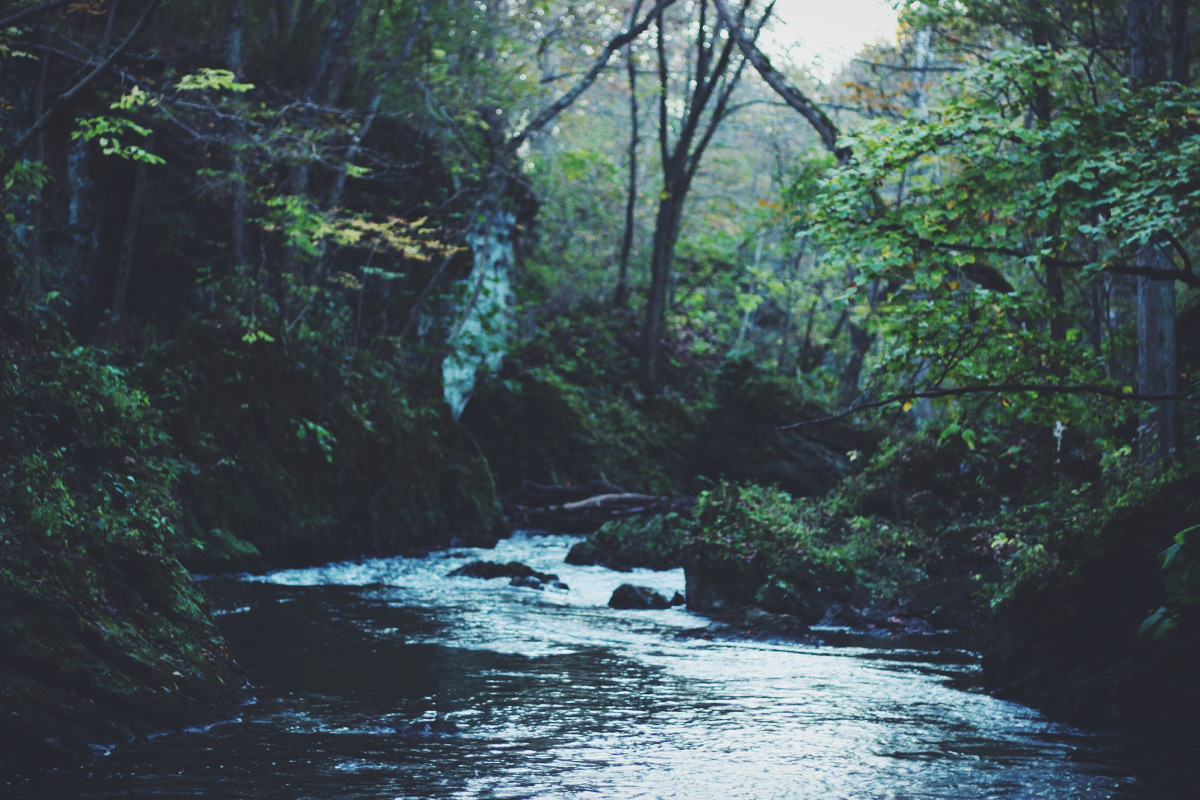
\includegraphics[width=\linewidth]{stream}
\caption{Legend (350 words max). Example legend text.}
\label{fig:stream}
\end{figure}

\begin{table}[ht]
\centering
\begin{tabular}{|l|l|l|}
\hline
Condition & n & p \\
\hline
A & 5 & 0.1 \\
\hline
B & 10 & 0.01 \\
\hline
\end{tabular}
\caption{\label{tab:example}Legend (350 words max). Example legend text.}
\end{table}

Figures and tables can be referenced in LaTeX using the ref command, e.g. Figure \ref{fig:stream} and Table \ref{tab:example}.

\end{document}